\documentclass[10pt]{article}
\usepackage[margin=1in]{geometry}
\usepackage{graphicx}
\graphicspath{{D:/MASTER/5th_Semester/Legacy_contamination/Exercises_(English)/final_submission/revision/figures}}
\usepackage{subcaption}
\usepackage{amsmath}
\usepackage{float}
\usepackage{cite}
\usepackage{caption}
\usepackage{booktabs}
\usepackage{parskip}
\usepackage{tikz}
\usepackage{epstopdf}

\title{Exercise: Identification of Pollution Concentrations in a Shallow Groundwater Aquifer using Data-Driven Approaches}
\author{Roger Roca Miró \\ Legacy Contamination and Soil Remediation \\ TU Bergakademie Freiberg}
\date{\today}

\usepackage{titling}
\setlength{\droptitle}{-60pt}

\begin{document}
	
	\maketitle
	
	\section{Introduction}
	Groundwater contamination is a critical issue with significant environmental and public health implications. Accurate prediction of pollutant concentrations is essential for effective remediation and risk management. In this report, we apply the methodology of Taherdangkoo et al. \cite{taherdangkoo2020} by adapting feedforward neural network (FFNN) training algorithms—Levenberg–Marquardt (LM) and Bayesian Regularization (BR).

	The LM algorithm, introduced by Hagan and Menhaj (1994), is recognized for its computational efficiency and rapid convergence when training FFNN. MATLAB implements this algorithm in the \texttt{trainlm} function, which has become one of the most widely used tools for training neural networks due to its reliability and speed \cite{hagan1994,matlab}.

	The Bayesian Regularization algorithm, detailed by Foresee and Hagan (1997) \cite{foresee1997,matlab}, enhances model generalization through a Bayesian probabilistic framework. Its implementation in MATLAB as the \texttt{trainbr} function integrates the training and validation phases, providing an optimal solution for limited datasets common in groundwater contamination scenarios. This method reduces the risk of overfitting by automatically adjusting regularization parameters during training, effectively improving predictive accuracy and robustness.

	Our approach simulates contaminant migration in a shallow groundwater aquifer and compares the performance of both algorithms while evaluating the influence of key hydrogeological parameters using MATLAB.
	
	\section{Methodology}
	\subsection{Conceptual Model and Boundary Conditions}
	The 2D generic contamination model domain spans 150 m in length and 100 m in width, and is set to be located at a depth of 30 m (depth being just relevant to make clear that it represents a shallow aquifer). Two leakage sources are positioned along the left boundary, while an observation well is placed on the right side of the domain. The key input parameters for the simplified model are \textit{permeability}, \textit{porosity}, and \textit{layer length}, while the output is the contaminant concentration.
	
	Groundwater flows from left to right under single-phase flow conditions, with the contaminant treated as a conservative tracer (i.e., sorption and degradation processes are neglected). Pressure head boundaries are applied laterally, and no-flow conditions are enforced at the top and bottom boundaries. All strata are assumed to be homogeneous and isotropic.
	The contaminant is allowed to leak into the aquifer over a simulation period of 150 hours. \textit{Figure \ref{fig:contamination_model}} presents a detailed diagram of the proposed model.
	
	\begin{figure}[h]
		\centering
		\begin{tikzpicture}
			
			% Draw the rectangular domain
			\fill[gray!50] (0,0) rectangle (15,10);
			
			% Draw the vertical partitions
			\draw (5,0) -- (5,10);
			\draw (10,0) -- (10,10);
			
			% Draw sources and observation well
			\fill (2.5,3) circle (0.15);  % Source 1
			\fill (2.5,7) circle (0.15);  % Source 2
			\fill (12.5,5) circle (0.15); % Observation well
			
			% Add labels ABOVE the dots with some vertical separation
			\node[above=5pt, red] at (2.5,3) {\textbf{Source 1}};
			\node[above=5pt, red] at (2.5,7) {\textbf{Source 2}};
			\node[above=5pt, green] at (12.5,5) {\textbf{Observation well}};
			
			% Axes and dimensions
			\draw[thick, ->] (-0.5,0) -- (-0.5,10);
			\draw[thick, ->] (0,-0.5) -- (15,-0.5);
			
			% Rotated label for width
			\node[rotate=90] at (-1.2,5) {\textbf{Width = 100 m}};
			
			% Label for length
			\node at (7.5,-1) {\textbf{Length = 150 m}};
			
		\end{tikzpicture}
		\caption{\textit{2D generic contamination model to investigate flow and transport of contaminant plumes in a shallow aquifer. Modified in \LaTeX{} from the WS 2023 Prof. Taherdangkoo slides.}}
		\label{fig:contamination_model}
	\end{figure}
	
	\subsection{Neural Network Structures and Training Algorithms}
	
	A FFNN with one hidden layer is employed to predict pollutant concentrations in shallow aquifers. Similar neural network structures have been applied in recent groundwater contamination studies by Sandra M. Guzman et. al. (2017) \cite{guzman2017}. and Taherdangkoo et. al. (2020) \cite{taherdangkoo2020}. 
	
	\newpage
	
		\underline{\textit{Data Normalization and Division}} \\
		\\
		Input and target data are normalized to the range  using the \textit{mapminmax} function, since training algorithms typically perform better with data centered at zero \cite{guzman2017,taherdangkoo2020}. The dataset is split into training (70\%), validation (15\%), and testing (15\%).
		
		\underline{\textit{Network Architecture}} \\
		\\
		The hidden layer uses a hyperbolic tangent sigmoid (\textit{tansig}) \cite{matlab-tansig} transfer function, chosen over the default \textit{logsig} \cite{matlab-logsig} due to the normalized data range of \([-1, 1]\). The output layer applies a linear transfer function to facilitate continuous-value prediction.
		
		\underline{\textit{Training Algorithms}} \\
		\\
		As explained earlier, the two algorithms used are the LM and the BR. LM algorithm is favored in the field, for fast convergence and efficiency, particularly in scenarios requiring rapid training and reliable predictions \cite{taherdangkoo2020}.
		
		Regarding the FFNN-BR, which often integrates training and validation sets, enhancing generalization \cite{guzman2017,taherdangkoo2020,foresee1997}, we still separated the validation set. The reason was to ensure that both algorithms were evaluated under the same conditions. The validation partition is effectively inert for stopping in the BR case, but it still allows us to compute an even validation error metric for both algorithms.
		
		\newpage
		
		
		\underline{\textit{Performance Evaluation}} \\
		\\
		Model performance is assessed via performance metrics. The MSE, RMSE and $R^{2}$ are computed separately on the training, validation and test sets, per every number of neurons defining every model. The model yielding the lowest validation MSE is identified as the best model for each algorithm.
		
		\underline{\textit{Parameter Importance Analysis}} \\
		\\
		The Leave-One-Variable-Out (LOVO) method is executed in the code by systematically removing each input variable (\textit{permeability}, \textit{porosity}, and \textit{layer length}) and retraining the best FFNN (previously selected depending on the validation MSE, as explained earlier) without that specific parameter. The method is simplified from J. D. Olden et. al. (2004) \cite{olden2004}. The performance degradation is quantified by computing the mean squared error (MSE) for training and testing datasets. The impact of each parameter is measured by averaging these MSE differences and normalizing them to derive a relative importance metric. Finally, a bar chart is generated to visualize the normalized contribution of each parameter, aiding in the interpretation of their influence on the model's predictions. Validation MSE is not included in this step, as it is primarily used for model selection rather than importance quantification. Including it could introduce bias, since the validation set is already involved in tuning the best FFNN, potentially leading to an overestimation or underestimation of parameter importance due to prior model adjustments. 
	
	\section{Results and Discussion}
	
	Both FFNN-LM and FFNN-BR demonstrated strong predictive capabilities when trained on normalized data. The FFNN-LM achieved its best performance using 30 neurons (Training MSE: \(8.77 \times 10^3\), Validation MSE: \(4.42 \times 10^4\), Testing MSE: \(1.04 \times 10^5\)), while the FFNN-BR performed optimally with 13 neurons (Training MSE: \(2.45 \times 10^4\), Validation MSE: \(4.23 \times 10^4\), Testing MSE: \(4.57 \times 10^4\)). These results indicate that the FFNN-BR generally outperformed the FFNN-LM, particularly in terms of testing error and number of neurons.
	
	To provide a more comprehensive assessment of predictive performance, additional evaluation metrics, including Root Mean Squared Error (RMSE) and the coefficient of determination ($R^2$), were computed.
	
	\textit{Figure \ref{fig:comparisonMSE}} presents the performance comparison between the FFNN-LM and FFNN-BR algorithms in terms of MSE as a function of the number of neurons. The results indicate that while LM achieves lower training error, the BR network exhibits superior generalization capabilities. In this graph, FFNN-LM obtains the highest peaks of MSE, especially for the testing dataset.
	
	\textit{Figure \ref{fig:comparisonRMSE}} and \textit{Figure \ref{fig:comparisonR2}} illustrate similar trends for RMSE and $R^2$ metrics. The RMSE comparison reveals that the BR network maintains lower error values across all tested neuron configurations, better than \textit{Figure \ref{fig:comparisonMSE}}. Likewise, \textit{Figure \ref{fig:comparisonR2}} confirms that the BR network achieves higher $R^2$ values, signifying a stronger correlation between predicted and actual pollutant concentrations, also making the trends clearer than \textit{Figure \ref{fig:comparisonMSE}}. These graphs also support the selection criteria for the optimal model based on validation error. While alternative FFNN configurations, particularly LM with a lower number of neurons, could have been considered, our final choice remains justified, especially when evaluating the validation functions.
	
	\begin{figure}[H]
		\centering
		\includegraphics[width=0.8\textwidth]{MSE\_neurons.eps}
		\caption{\textit{Algorithm Performance Comparison: MSE vs. number of neurons for the FFNN-LM and FFNN-BR. Circular markers indicate the best-performing networks for each algorithm, pointing on the validation dataset line.}}
		\label{fig:comparisonMSE}
	\end{figure}
	
	\begin{figure}[H]
		\centering
		\includegraphics[width=0.8\textwidth]{RMSE\_neurons.eps}
		\caption{\textit{Algorithm Performance Comparison: RMSE vs. number of neurons for the FFNN-LM and FFNN-BR. Circular markers indicate the best-performing networks for each algorithm, pointing on the validation dataset line.}}
		\label{fig:comparisonRMSE}
	\end{figure}
	
	\begin{figure}[H]
		\centering
		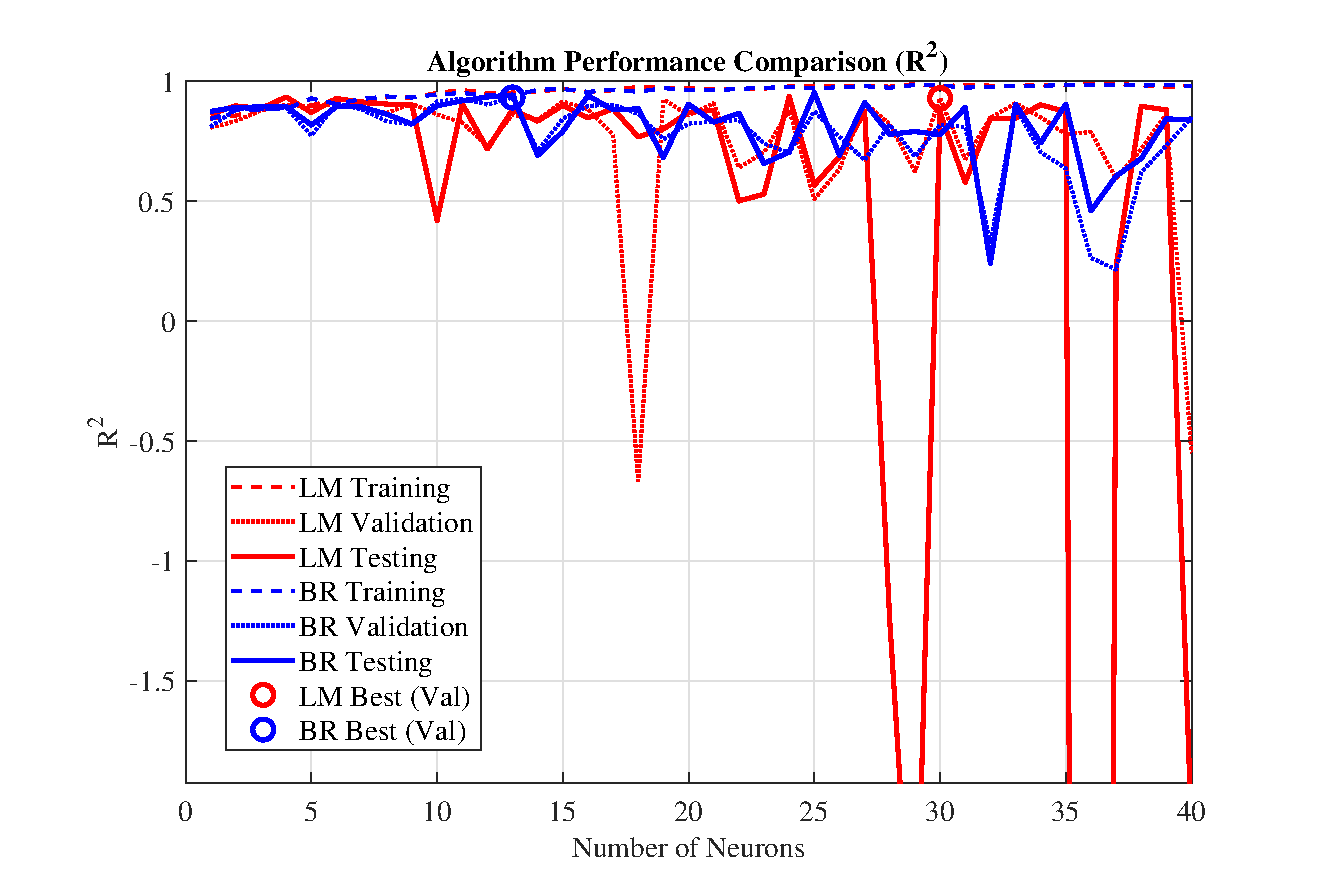
\includegraphics[width=0.8\textwidth]{R-2_neurons.eps}
		\caption{\textit{Algorithm Performance Comparison: \(R^2\) vs. number of neurons for the FFNN-LM and FFNN-BR. Circular markers indicate the best-performing networks for each algorithm, pointing on the validation dataset line.}}
		\label{fig:comparisonR2}
	\end{figure}
	
	The regression analyses for the FFNN-LM and FFNN-BR, depicted in \textit{Figure \ref{fig:lm_sct}} and \textit{Figure \ref{fig:br_sct}}, respectively, provide further insights into model performance. For the FFNN-LM (\textit{Figure \ref{fig:lm_sct}}), scatter plots of true versus predicted values indicate a strong correlation along the 45-degree line, though larger discrepancies appear in the validation and testing datasets. Similarly, \textit{Figure \ref{fig:br_sct}} shows that the BR network exhibits better agreement between predicted and actual pollutant concentrations, confirming its superior predictive accuracy. The FFNN-LM also performs worse regarding extreme values, this is best observed from the 2000 line onwards, in both axis, where 9 outliers are identified in the testing dataset (with its particular importance, since it doesn't train the FFNNs).
	
	\begin{figure}[H]
		\centering
		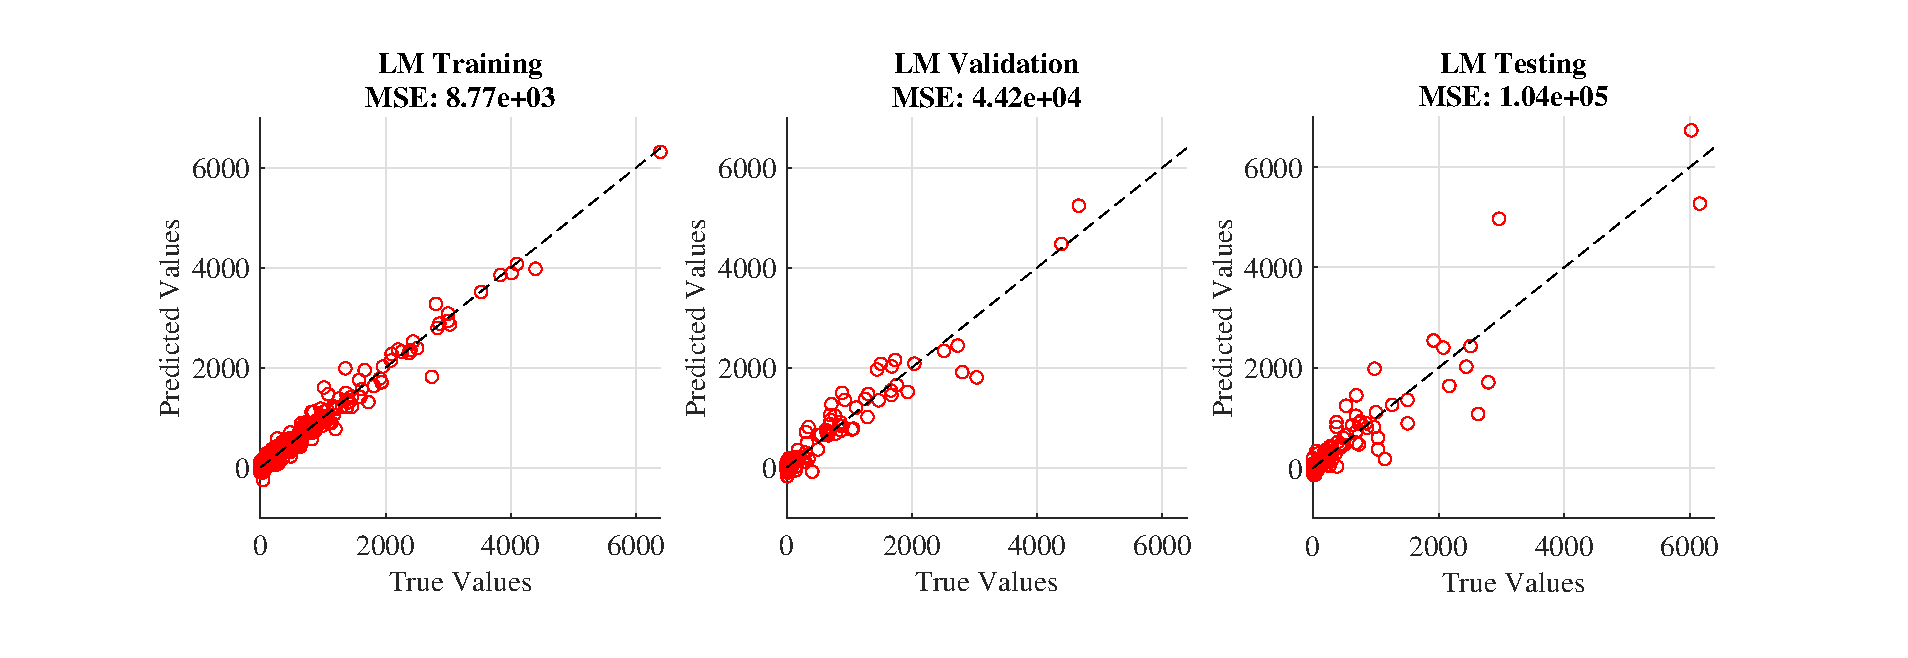
\includegraphics[width=1\textwidth]{LM_scatterplots.eps}
		\caption{\textit{LM Network Regression Analysis: Scatter plots for (a) training, (b) validation, and (c) testing datasets with corresponding MSE values.}}
		\label{fig:lm_sct}
	\end{figure}
	
	\begin{figure}[H]
		\centering
		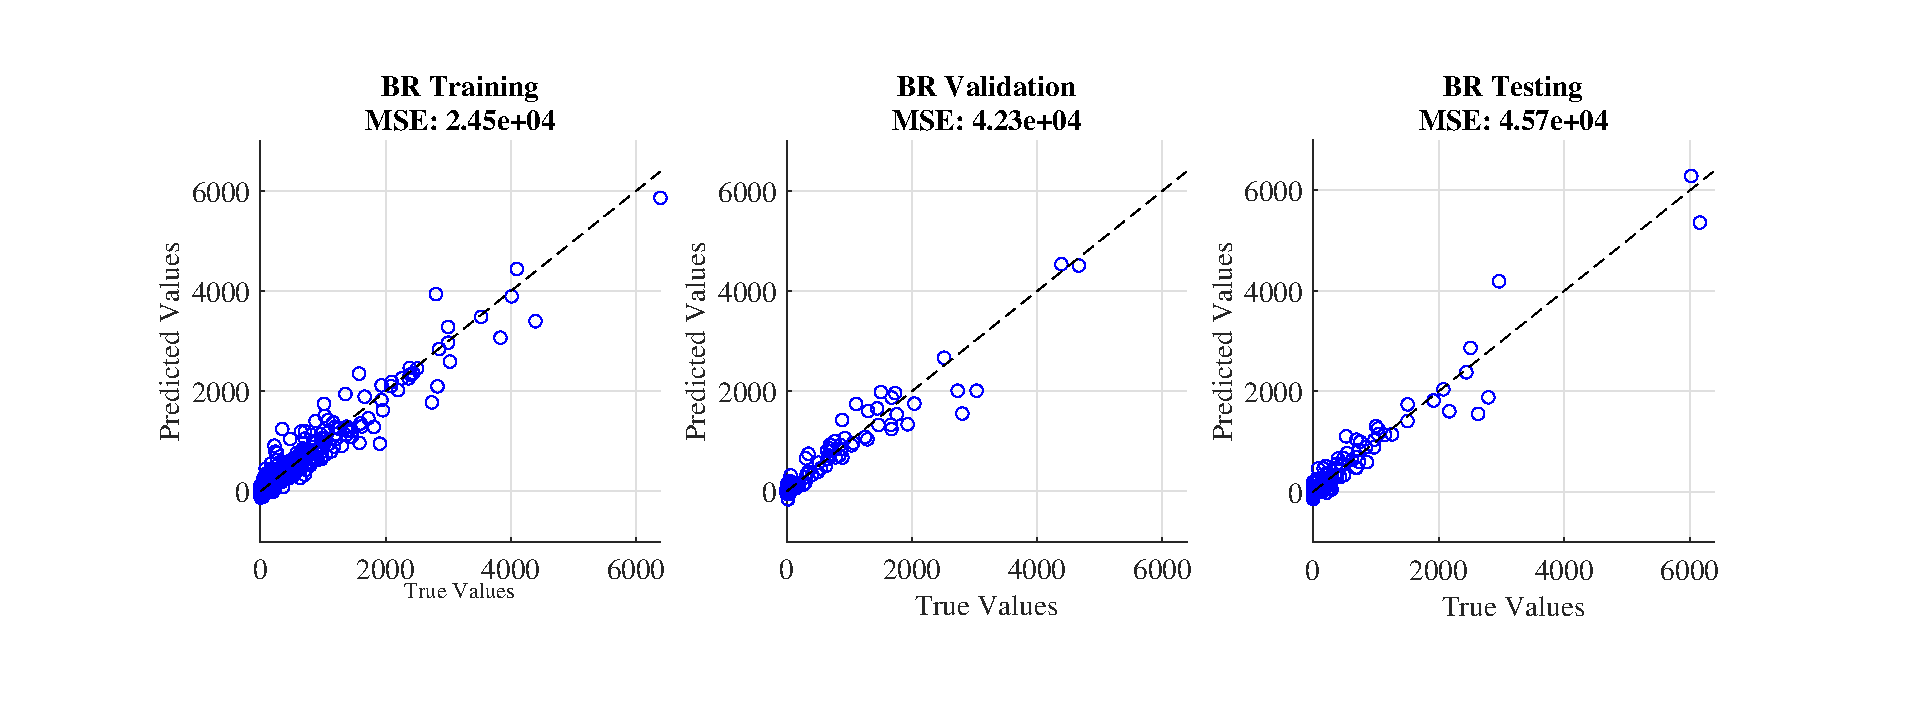
\includegraphics[width=1\textwidth]{BR_scatterplots.eps}
		\caption{\textit{BR Network Regression Analysis: Scatter plots for (a) training, (b) validation, and (c) testing datasets with corresponding MSE values.}}
		\label{fig:br_sct}
	\end{figure}
	
	To assess parameter importance, a sensitivity analysis was conducted. The bar chart in \textit{Figure \ref{fig:param_imp}} reveals that \textit{porosity} is the most influential parameter (normalized importance: 0.543), followed by \textit{layer length} (0.281) and \textit{permeability} (0.176). These findings underscore the dominant role of \textit{porosity} in determining pollutant dispersion, while \textit{permeability} and \textit{layer length} remain significant secondary contributors.
	
	\begin{figure}[H]
		\centering
		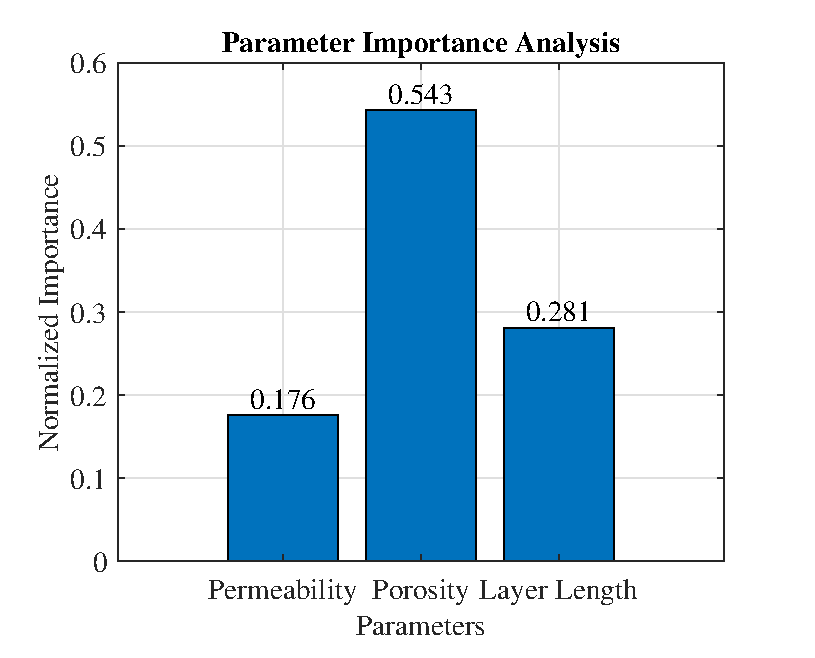
\includegraphics[width=0.6\textwidth]{parameter_importance.eps}
		\caption{\textit{Parameter Importance Analysis: Normalized importance of input parameters obtained by evaluating the impact of each parameter's exclusion on network performance.}}
		\label{fig:param_imp}
	\end{figure}
	
	\section{Conclusion}
	This study has demonstrated the application of data-driven neural network approaches for the prediction of pollution concentrations in a shallow groundwater aquifer. A two-dimensional contamination model was employed to simulate pollutant transport under realistic boundary conditions. Neural networks with varying numbers of hidden neurons were trained using both Levenberg-Marquardt and Bayesian Regularization algorithms.
	
	Both LM and BR networks provided accurate predictions, but the results clearly indicate that the BR algorithm is the superior choice for this application in all ambits (less number of neurons, and less MSE, RMSE and higher $R^2$ across testing datasets). The FFNN-LM performance was optimized by monitoring validation MSE, while the BR network benefited from an automatic regularization mechanism, enhancing its generalization ability.
	
	The parameter importance analysis confirmed that \textit{porosity} is the most significant predictor of pollution spread, while \textit{permeability} and \textit{layer length} also play important roles. These findings provide valuable insights into groundwater contamination modelling and suggest that BR-based feedforward neural networks are well-suited for predictive environmental analysis.
	
	% References
	\bibliographystyle{apalike}
	
	\begin{thebibliography}{99} % 99 is the widest label (adjust as needed)
		\bibitem{foresee1997}
		Foresee, F. D., \& Hagan, M. T. (1997). Gauss–Newton approximation to Bayesian learning. In Proceedings of International Conference on Neural Networks (ICNN’97) (Vol. 3, pp. 1930–1935). IEEE. https://doi.org/10.1109/ICNN.1997.614194
		\bibitem{guzman2017}
		Guzman, Sandra M.; Paz, Joel O.; Tagert, Mary Love M. (2017): The Use of NARX Neural Networks to Forecast Daily Groundwater Levels. In Water Resour Manage 31 (5), pp. 1591–1603. DOI: 10.1007/s11269-017-1598-5.
		\bibitem{hagan1994}
		Hagan, M. T., \& Menhaj, M. B. (1994). Training feedforward networks with the Marquardt algorithm. IEEE Transactions on Neural Networks, 5(6), 989–993. https://doi.org/10.1109/72.329697
		\bibitem{matlab}
		MathWorks. (n.d.). Choose a multilayer neural network training function. MATLAB Documentation. Retrieved March 7, 2025, from https://www.mathworks.com/help/deeplearning/ug/choose-a-multilayer-neural-network-training-function.html
		\bibitem{matlab-tansig}
		MathWorks (n.d.). tansig: Hyperbolic tangent sigmoid transfer function. Retrieved from https://de.mathworks.com/help/deeplearning/ref/tansig.html.
		\bibitem{matlab-logsig}
		MathWorks (n.d.). logsig: Log-sigmoid transfer function. Retrieved from https://de.mathworks.com/help/deeplearning/ref/logsig.html.
		\bibitem{olden2004}
		Olden, J. D., Joy, M. K., \& Death, R. G. (2004). An accurate comparison of methods for quantifying variable importance in artificial neural networks using simulated data. Ecological Modelling, 178(3–4), 389–397.
		\bibitem{taherdangkoo2020}
		Taherdangkoo, R., Tatomir, A., Taherdangkoo, M., Qiu, P., \& Sauter, M. (2020). Nonlinear autoregressive neural networks to predict hydraulic fracturing fluid leakage into shallow groundwater. Water, 12(3), 841. https://doi.org/10.3390/w12030841
	\end{thebibliography}
	
\end{document}
